\documentclass[reprint, amsmath,amssymb,aps,pre,onecolumn,notitlepage%,superscriptaddress
]{revtex4-1}
\usepackage{subfigure}
\usepackage{graphicx}
\usepackage{mathtools,amsmath}
%\usepackage[mathlines]{lineno}
%\linenumbers\relax
\usepackage{amssymb}
\usepackage{float}
\usepackage{graphicx}
\usepackage{subfigure,bm}
\usepackage[export]{adjustbox}
\usepackage{type1cm}
\usepackage{color,natbib}
\usepackage{empheq,wrapfig}
\begin{document}

\preprint{APS/123-QED}
\title{Lubrication Forces}
\author{Ranga}
\affiliation{University of Edinburgh, UK}
\pacs{Valid PACS appear here}
\date{\today}

% =============================================

\maketitle

\section{Computing forces and torques}


\begin{wrapfigure}{r}{6cm}
	\centering
	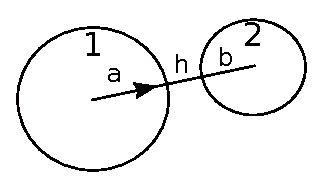
\includegraphics[width=5cm]{drawing.eps}
	\caption{Sketch of the two spheres with the normal vector indicated by the arrow.}
	\label{fig:sketch}
\end{wrapfigure}

The lubrication force between a pair of particles (say $p=1,q=2$) are given as a product between the Grand Resistance Matrix, which only depends on the positions of the two particles, and a vector containing particle and background fluid velocities in Refs.~\cite{J1992, KK1991,Mari2014}. Our task below is to simplify the relation between the lubrication forces and torques given in Refs.~\cite{J1992, KK1991,Mari2014} for spheres of different sizes into a form similar to the one given by Ball\&Melrose for spheres of the same size~\cite{Ball1997}. \\

We have sphere $p=1$ of radius a at position $\vec{x}^1$, separated by a distance h from sphere $q=2$ of radius b at position $\vec{x}^2$ as shown in Fig.~\ref{fig:sketch}. The superscripts denote the particle number, and later the subscript will denote the component index. The total center to center distance is given by $R=|\vec{x}^1-\vec{x}^2|=a+b+h$. The separation between the two spheres is non-dimensionalised as
\begin{equation}
	\xi=\frac{2(R-a-b)}{a+b}=\frac{h}{(a+b)/2} \ ,
\end{equation}
and the normal vector connecting the two spheres is given by
\begin{equation}
	\vec{n}=\frac{\vec{x}^2-\vec{x}^1}{|\vec{x}^2-\vec{x}^1|}=\frac{\vec{x}^2-\vec{x}^1}{R}\ .
\end{equation}
The velocity vectors of the spheres are given by $\vec{U}^1,\vec{U}^2}$, and the angular velocities by $\vec{\omega}^1,\vec{\omega}^2$. The background fluid velocity is assumed to be linear with uniform velocity given by $\vec{v}^\infty$, angular velocity given by $\vec{\Omega}^\infty$, and rate of strain tensor given by $\bm{E^\infty}$.\\ 

According to Ref. \cite{KK1991}, the lubrication force acting on sphere 1 is given by
\begin{equation}
	\begin{split}
		F^1/\mu=& \bm{A}^{11}(\vec{v}^\infty(\vec{x^1})-\vec{U}^1)+\bm{A}^{12}(\vec{v}^\infty(\vec{x}^2)-\vec{U^2})\\
		&+ \widetilde{\bm{B}}^{11}(\vec{\Omega}^\infty-\vec{\omega}^1)+\widetilde{\bm{B}}^{12}(\vec{\Omega}^\infty-\vec{\omega}^2)\\
		&+ \widetilde{\bm{G}}^{11}\bm{E}^\infty + \widetilde{\bm{G}}^{12}\bm{E}^\infty \ ,
	\end{split}
	\label{eq:force1}
\end{equation}
and the torque is given by
\begin{equation}
	\begin{split}
		T^1/\mu=& \bm{B}^{11}(\vec{v}^\infty(\vec{x^1})-\vec{U}^1)+\bm{B}^{12}(\vec{v}^\infty(\vec{x}^2)-\vec{U^2})\\
		&+ \widetilde{\bm{C}}^{11}(\vec{\Omega}^\infty-\vec{\omega}^1)+\widetilde{\bm{C}}^{12}(\vec{\Omega}^\infty-\vec{\omega}^2)\\
		&+ \widetilde{\bm{H}}^{11}\bm{E}^\infty + \widetilde{\bm{H}}^{12}\bm{E}^\infty \ ,
	\end{split}
	\label{eq:torque1}
\end{equation}
where the bold symbols denote resistance functions which operate on a vector, say $\vec{\chi}=\chi_j$, as specified below
\begin{equation}
	\begin{split}
		A^{pq}_{ij}&=X_A^{pq}n_in_j+Y_A^{pq}(\delta_{ij}-n_in_j)\ ,\\
		B^{pq}_{ij}&=Y_B^{pq}\epsilon_{ijk}n_k\ ,\\
		C^{pq}_{ij}&=X_C^{pq}n_in_j+Y_C^{pq}(\delta_{ij}-n_in_j)\ ,\\
		G^{pq}_{ijk}&=X_G^{pq}(n_in_j-\delta_{ij}/3)n_k+Y_G^{pq}(n_i\delta_{jk}+n_j\delta_{ik}-2n_in_jn_k)\\
		H^{pq}_{ijk}&=Y_H^{pq}(\epsilon_{ikl} n_l n_j+\epsilon_{jkl} n_l n_i)\ .
	\end{split}
	\label{eq:x_terms}
\end{equation}
Further, $\widetilde{B}^{pq}_{ij}=B^{qp}_{ji}$, $\widetilde{G}^{pq}_{ijk}=G^{qp}_{jki}$, $\widetilde{H}^{pq}_{ijk}=H^{qp}_{jki}$ are required due to symmetry reasons of the resistance matrix formulation. Therefore, we also have
\begin{equation}
	\begin{split}
		\widetilde{B}^{11}_{ij}=B^{11}_{ji}&=-Y_B^{11}\epsilon_{ijk}n_k\ ,\\
		\widetilde{B}^{12}_{ij}=B^{21}_{ji}&=-Y_B^{21}\epsilon_{ijk}n_k\ ,\\
		\widetilde{G}^{11}_{ijk}=G^{11}_{jki}&=X_G^{11}(n_jn_k-\delta_{jk}/3)n_i+Y_G^{11}(n_j\delta_{ki}+n_k\delta_{ji}-2n_jn_kn_i)\ ,\\
		\widetilde{G}^{12}_{ijk}=G^{21}_{jki}&=X_G^{21}(n_jn_k-\delta_{jk}/3)n_i+Y_G^{21}(n_j\delta_{ki}+n_k\delta_{ji}-2n_jn_kn_i)\ ,\\
		\widetilde{H}^{11}_{ijk}=H^{11}_{jki}&=-Y_H^{11}(\epsilon_{ijl} n_l n_k+\epsilon_{ikl} n_l n_j)\ ,\\
		\widetilde{H}^{12}_{ijk}=H^{21}_{jki}&=-Y_H^{21}(\epsilon_{ijl} n_l n_k+\epsilon_{ikl} n_l n_j)\ .
	\end{split}
\end{equation}
The different components of the resistance functions specified by symbols such as $X_A^{pq},Y_A^{pq},\ldots$ are given in Sec.~\ref{sec:components}, and the relations between them are specified in Eq.~\eqref{eq:relations}.  It follows that the lubrication force given in Eq.~\eqref{eq:force1} can be written in component form as
\begin{equation}
	\begin{split}
		F^1_i/\mu=& (\ X_A^{11}n_in_j+Y_A^{11}(\delta_{ij}-n_in_j)\ )(U^2_j-U^1_j)\\
		&-\epsilon_{ijk} \left(Y_B^{11}(\Omega_j^\infty-\omega_j^1)+Y_B^{21}(\Omega_j^\infty-\omega_j^2)\right) n_k\\
& +(\ X_A^{11}n_in_j+Y_A^{11}(\delta_{ij}-n_in_j)\ )(v_j^\infty(x^1)-v_j^\infty(x^2))\\
		&+(X_G^{11}+X_G^{21})(n_jn_k-\delta_{jk}/3)n_iE^\infty_{jk}\\
		&+(Y_G^{11}+Y_G^{21})(n_j\delta_{ki}+n_k\delta_{ji}-2n_jn_kn_i)E^\infty_{jk}\ , 
	\end{split}
	\label{eq:force}
\end{equation}
and the torque given by Eq.~\eqref{eq:torque1} in component form is
\begin{equation}
	\begin{split}
		T^1_i/\mu=& \epsilon_{ijk}Y_B^{11}(U^2_j-U^1_j)n_k\\
		&-\epsilon_{ijk}Y_B^{11}(v^\infty_j(x_2)-v^\infty_j(x_1))n_k\\
		&+(\delta_{ij}-n_in_j)\left(Y_C^{11}(\Omega^\infty_j-\omega^1_j)+Y_C^{12}(\Omega^\infty_j-\omega^2_j)\right)\ ,\\
		&- (Y^{11}_H+Y^{21}_H)(\epsilon_{ijl} n_l n_k+\epsilon_{ikl} n_l n_j) E^\infty_{jk}\ .
	\end{split}
	\label{eq:t1_comp}
\end{equation}

Our objective is to make use of the relations between the different terms in Eq.~\eqref{eq:relations} and the simplifications in Sec.~\ref{sec:simple} to convert the forces and torques above into simpler forms.

\newpage
\section{Computing the force acting on the spheres}
\subsection{Grouping terms in Eq.~\eqref{eq:force}}
\label{sec:forcegroup}
Making use of the relations in Eq.~\eqref{eq:relations}, and Sec.~\ref{sec:simple}, we can get
\begin{equation}
\begin{split}
 X_A^{11}n_in_j(v_j^\infty(x^1)-v_j^\infty(x^2)) +(X_G^{11}+X_G^{21})(n_jn_k-\delta_{jk}/3)n_iE^\infty_{jk}=& X_A^{11}E^\infty_{jk}n_i n_j n_k  (-R+a+b)\\
 &=-X_A^{11} E^\infty_{jk}n_i n_j n_k (a+b) (\xi/2)\approx 0
\end{split}
\end{equation}


\begin{equation}
\begin{split}
Y_A^{11}&(\delta_{ij}-n_in_j)(v_j^\infty(x^1)-v_j^\infty(x^2)) +(Y_G^{11}+Y_G^{21})(n_j\delta_{ki}+n_k\delta_{ji}-2n_jn_kn_i)E^\infty_{jk} \\
=&-Y^{11}_A\left((\delta_{ij}-n_in_j)E^\infty_{jk}n_k +\epsilon_{ikl}\Omega^\infty_k n_l \right)R+Y_A^{11}(\delta_{ij}-n_in_j)n_kE^\infty_{jk}(a+b)\\
=&-Y^{11}_A\epsilon_{ikl}\Omega^\infty_k n_l R - Y^{11}_A(\delta_{ij}-n_in_j)E^\infty_{jk}n_k (a+b) \xi/2 \\
\approx&-Y^{11}_A\epsilon_{ikl}\Omega^\infty_k n_l R 
\end{split}
\end{equation}

\begin{equation}
\begin{split}
-Y^{11}_A\epsilon_{ijk}\Omega^\infty_j n_k R - (Y^{11}_B+Y^{21}_B)\epsilon_{ijk}\Omega^\infty_j n_k &=-Y^{11}_A\epsilon_{ijk}\Omega^\infty_j n_j (R-(a+b))\\
&=-Y^{11}_A\epsilon_{ijk}\Omega^\infty_j n_j(a+b) \xi/2 \approx 0
\end{split}
\end{equation}



\subsection{Simplified Lubrication force acting on sphere 1}
Using the results from Sec.~\ref{sec:forcegroup}, Eq.~\eqref{eq:force} simplifies to
\begin{empheq}[box=\fbox]{equation}
\begin{split}
	F^1_i/\mu=& (\ X_A^{11}n_in_j+Y_A^{11}(\delta_{ij}-n_in_j)\ )(U^2_j-U^1_j)\\
	&+\epsilon_{ijk} \left(Y_B^{11}\omega_j^1+Y_B^{21}\omega_j^2\right) n_k\ .\\
\end{split}
\label{eq:simple}
\end{empheq}

and Eq.\eqref{eq:simple} can be written as
\begin{empheq}[box=\fbox]{equation}
\begin{split}
	F^1_i/\mu=& (\ X_A^{11}n_in_j+Y_A^{11}(\delta_{ij}-n_in_j)\ )(U^2_j-U^1_j)\\
	&-\frac{a+b}{2}\epsilon_{ijk}Y_A^{11} (\omega_j^1+\omega_j^2) n_k+\left(1-\frac{b(a+4b)}{a(4a+b)}\right)Y_B^{11}\epsilon_{ijk} (\omega_j^1-\omega_j^2) n_k/2\ .\\
\end{split}
\label{eq:simple2}
\end{empheq}


\subsection{Force acting on sphere 2}
According to the form given by Ref.~\cite{KK1991}
\begin{equation}
	\begin{split}
		F^2/\mu=& \bm{A}^{21}\cdot(v^\infty(x^1)-U^1)+\bm{A}^{22}\cdot(v^\infty(x^2)-U^2)\\
		&+ \widetilde{\bm{B}}^{21}(\Omega^\infty-\omega^1)+\widetilde{\bm{B}}^{22}(\Omega^\infty-\omega^2)\\
		&+ \widetilde{\bm{G}}^{21}\bm{E}^\infty + \widetilde{\bm{G}}^{22}\bm{E}^\infty
	\end{split}
	\label{eq:force2}
\end{equation}

And similar to Eq.~\eqref{eq:force}, we can write Eq.~\eqref{eq:force2} after using the relations given in Eq.~\eqref{eq:relations} as

\begin{equation}
	\begin{split}
		F^2_i/\mu=& -(\ X_A^{11}n_in_j+Y_A^{11}(\delta_{ij}-n_in_j)\ )(U^2_j-U^1_j)\\
		&+\epsilon_{ijk} \left(Y_B^{11}(\Omega_j^\infty-\omega_j^1)+Y_B^{21}(\Omega_j^\infty-\omega_j^2)\right) n_k\\
& -(\ X_A^{11}n_in_j+Y_A^{11}(\delta_{ij}-n_in_j)\ )(v_j^\infty(x^1)-v_j^\infty(x^2))\\
		&-(X_G^{22}+X_G^{12})(n_jn_k-\delta_{jk}/3)n_iE^\infty_{jk}\\
		&-(Y_G^{22}+Y_G^{12})(n_j\delta_{ki}+n_k\delta_{ji}-2n_jn_kn_i)E^\infty_{jk}\ . 
	\end{split}
	\label{eq:f2}
\end{equation}

Comparing Eq.~\eqref{eq:force} and Eq.~\eqref{eq:f2}, we get $\boxed{F_i^2=-F_i^1}$.
\newpage
\section{Lubrication Torques}
\subsection{Grouping terms in Eq.~\eqref{eq:t1_comp}}
Making use of the relations in Eq.~\eqref{eq:relations}, and Sec.~\ref{sec:simple}, we can get
\begin{equation}
\begin{split}
- (Y^{11}_H+Y^{21}_H)(\epsilon_{ijl} n_l n_k+\epsilon_{ikl} n_l n_j) E^\infty_{jk}=&(a+b)Y_B^{11}\epsilon_{ijl} n_l n_k E^\infty_{jk},\\
(Y_C^{11}+Y_C^{12})(\delta_{ij}-n_in_j)\Omega_j^\infty =&-(a+b)Y_B^{11}(\delta_{ij}-n_in_j)\Omega_j^\infty \ ,\\
-Y_B^{11}\epsilon_{ijl}(v^\infty_j(x_2)-v^\infty_j(x_1))n_l=&-(a+b)(1+\xi/2)Y_B^{11}\left(\epsilon_{ijl}n_k n_l E^\infty_{jk}- (\delta_{ij}- n_i n_j)\Omega^\infty_j  \right)\ ,
\end{split}
\end{equation}
which implies that
\begin{equation}
	\begin{split}
(Y_C^{11}+Y_C^{12})(\delta_{ij}-n_in_j)\Omega_j^\infty -\epsilon_{ijk}Y_B^{11}(v^\infty_j(x_2)-v^\infty_j(x_1))n_k - (Y^{11}_H+Y^{21}_H)(\epsilon_{ijl} n_l n_k+\epsilon_{ikl} n_l n_j) E^\infty_{jk}\\= \xi (a+b) Y_B^{11}\left(\epsilon_{ijl}n_k n_l E^\infty_{jk}+ (\delta_{ij}- n_i n_j)\Omega^\infty_j  \right)/2 =\mathcal{O}(\xi)\approx 0 \ .
\end{split}
\end{equation}

\subsection{Torque acting on sphere 1}
Using the above equations, we get
\begin{equation}
		T^1_i/\mu=Y_B^{11}\epsilon_{ijk}(U^2_j-U^1_j)n_k-(\delta_{ij}-n_in_j)\left(Y_C^{11}\omega^1_j+Y_C^{12}\omega^2_j\right)\ .
\label{eq:tor1}
\end{equation}

We can try further simplification by noting
Therefore Eq.~\eqref{eq:tor1} becomes simply 
\begin{empheq}[box=\fbox]{equation}
	\begin{split}
		T^1_i/\mu=& Y_B^{11}\epsilon_{ijk}(U^2_j-U^1_j)n_k+(a+b)Y_B^{11}(\delta_{ij}-n_in_j)(\omega^1_j+\omega^2_j)/2\\
		&+(1-4a/b)Y_C^{12}(\delta_{ij}-n_in_j)(\omega^1_j-\omega^2_j)/2
	\end{split}
	\label{eq:t1_simp}
\end{empheq}
\subsection{Torque on sphere 2}
For the torque acting on sphere 2, we have 
\begin{equation}
	\begin{split}
		T^2/\mu=& \bm{B}^{21}(v^\infty(x^1)-U^1)+\bm{B}^{22}(v^\infty(x^2)-U^2)\\
		&+ \bm{C}^{21}(\Omega^\infty-\omega^1)+\bm{C}^{22}(\Omega^\infty-\omega^2)\\
		&+ \widetilde{\bm{H}}^{21}\bm{E}^\infty + \widetilde{\bm{H}}^{22}\bm{E}^\infty\ ,
	\end{split}
	\label{eq:torque2}
\end{equation}
which turns out to be
\begin{equation}
	\begin{split}
		T^2_i/\mu=& \epsilon_{ijk}Y_B^{21}(U^2_j-U^1_j)n_k\\
		&-\epsilon_{ijk}Y_B^{21}(v^\infty_j(x_2)-v^\infty_j(x_1))n_k\\
		&+(\delta_{ij}-n_in_j)\left(Y_C^{21}(\Omega^\infty_j-\omega^1_j)+Y_C^{22}(\Omega^\infty_j-\omega^2_j)\right)\ ,\\
		&- (Y^{22}_H+Y^{12}_H)(\epsilon_{ijl} n_l n_k+\epsilon_{ikl} n_l n_j) E^\infty_{jk}\ .
	\end{split}
	\label{eq:t2_comp}
\end{equation}

Analogous to the previous calculations, this makes Eq.~\eqref{eq:t2_comp} to be 
\begin{equation}
		T^2_i/\mu=Y_B^{21}\epsilon_{ijk}(U^2_j-U^1_j)n_k-(\delta_{ij}-n_in_j)\left(Y_C^{21}\omega^1_j+Y_C^{22}\omega^2_j\right)\ .
\label{eq:tor2}
\end{equation}
Therefore Eq.~\eqref{eq:tor2} becomes simply 
\begin{empheq}[box=\fbox]{equation}
	\begin{split}
		T^2_i/\mu=& Y_B^{21}\epsilon_{ijk}(U^2_j-U^1_j)n_k+(a+b)Y_B^{21}(\delta_{ij}-n_in_j)(\omega^1_j+\omega^2_j)/2\\
		&-(1-4b/a)(\delta_{ij}-n_in_j)Y_C^{21}(\omega^1_j-\omega^2_j)/2
	\end{split}
	\label{eq:t2_simp1}
\end{empheq}
Equally,
\begin{empheq}[box=\fbox]{equation}
	\begin{split}
		T^2_i/\mu=& \frac{b(a+4b)}{a(4a+b)}Y_B^{11}\epsilon_{ijk}(U^2_j-U^1_j)n_k+\frac{b(a+b)(a+4b)}{2a(b+4a)}Y_B^{11}(\delta_{ij}-n_in_j)(\omega^1_j+\omega^2_j)\\
		&-(1-4b/a)Y_C^{12}(\delta_{ij}-n_in_j)(\omega^1_j-\omega^2_j)/2
	\end{split}
	\label{eq:t2_simp2}
\end{empheq}


\section{Testing the simplified expressions}
\subsection{Comparison of the forces and torques to Ref.~\cite{Ball1997}}
For equal spheres, $b=a$, Eq.~\eqref{eq:simple2} for the force becomes
\begin{equation}
\begin{split}
	F^1_i/\mu=& (\ X_A^{11}n_in_j+Y_A^{11}(\delta_{ij}-n_in_j)\ )(U^2_j-U^1_j) -\epsilon_{ijk} Y_A^{11} a \left( \omega_j^1+ \omega_j^2\right) n_k\\
	=&-\left(\ X_A^{11}n_in_j+Y_A^{11}(\delta_{ij}-n_in_j)\ \right)\left( U^1_j+a(\vec{\omega}^1\times\vec{n})_j -(U^2_j-a(\vec{\omega}^2\times\vec{n})_j)\right) \ .\\
\end{split}
\label{eq:bm}
\end{equation}
and is equal to the form given in Ref.~\cite{Ball1997}.

For the torques, we have
\begin{empheq}{align*}
	T^1_i/\mu=& -aY_A^{11}\epsilon_{ijk}(U^2_j-U^1_j)n_k-a^2Y_A^{11}(\delta_{ij}-n_in_j)(\omega^1_j+\omega^2_j)\\
		&-3Y_C^{12}(\delta_{ij}-n_in_j)(\omega^1_j-\omega^2_j)/2\ , \\
	T^2_i/\mu=& -aY_A^{11}\epsilon_{ijk}(U^2_j-U^1_j)n_k-a^2Y_A^{11}(\delta_{ij}-n_in_j)(\omega^1_j+\omega^2_j)\\
		&+3Y_C^{12}(\delta_{ij}-n_in_j)(\omega^1_j-\omega^2_j)/2\ . 
\end{empheq}
The first two terms are the same as Ref.~\cite{Ball1997}. However, the third term is
\[
	3 Y_C^{12}/2=\frac{3}{5}\pi a^3 \ln(1/\xi) \ ,
\]
which is 4 times the value given in Ref.~\cite{Ball1997}.

\subsection{Shearing motion of two rigid surfaces}
\begin{wrapfigure}{r}{4cm}
	\centering
	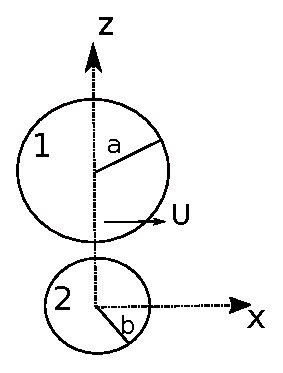
\includegraphics[width=3cm]{prob1.eps}
	\caption{Sketch of the two spheres with the normal vector indicated by the arrow.}
	\label{fig:sketch1}
\end{wrapfigure}
This is an example problem in Chap. 9 of Ref.~\cite{KK1991}. Sphere 1 is moving past a fixed sphere 2 along the x-axis at a constant velocity U. We have $\vec{U}^1=U \hat{x}$, $\vec{U}^2=0$, $\vec{\omega}^1=0$, $\vec{\omega}^2=0$, and $\vec{v}_\infty=0$ . 

The force on particle 1 given by Eq.~\eqref{eq:simple} after substituting for the different values of velocities becomes 
\begin{equation}
	F^1_x=-\mu Y_A^{11}U\ ,
\end{equation}
and after substituting for $Y_A^{11}$ from Sec.~\ref{sec:components}, we get
\begin{equation}
	\frac{F^1_x}{6 \pi \mu a U}=-\frac{4 \beta (2+  \beta + 2\beta^2)}{15 (1+\beta)^3} \ln{\xi^{-1}} \ .
\end{equation}

The torque on particle 1 given by Eq.~\eqref{eq:tor1} after substituting for the different values of velocities becomes 
\begin{equation}
	T^1_y=-\mu Y_B^{11}U\ ,
\end{equation}
and after substituting for $Y_B^{11}$ from Sec.~\ref{sec:components}, we get
\begin{equation}
	\frac{T^1_y}{ 8 \pi \mu a^2 U}= \frac{ \beta (4+ \beta)}{10 (1+\beta)^2} \ln{\xi^{-1}}\ .
\end{equation}
These results are the same as that Eq. (9.24), Eq. (9.25) in Ref.~\cite{KK1991}.

\newpage

\subsection{Shearing motion of two rigid surfaces due to rotation}
\begin{wrapfigure}{r}{4cm}
	\centering
	\includegraphics[width=3cm]{prob2.eps}
	\caption{Sketch of the two spheres with the normal vector indicated by the arrow.}
	\label{fig:sketch2}
\end{wrapfigure}
This is an example problem in Chap. 9 of Ref.~\cite{KK1991}. Sphere 1 is rotating near a fixed sphere 2 about the y-axis at a constant angular velocity $\omega$. We have $\vec{U}^1=0$, $\vec{U}^2=0$, $\vec{\omega}^1= \omega \hat{y}$, $\vec{\omega}^2=0$, and $\vec{v}_\infty=0$ . 

The force on particle 1 given by Eq.~\eqref{eq:simple} after substituting for the different values of velocities becomes 
\begin{equation}
	F^1_x=-\mu Y_B^{11}\omega \ ,
\end{equation}
and after substituting for $Y_B^{11}$ from Sec.~\ref{sec:components}, we get
\begin{equation}
	\frac{F^1_x}{ 8 \pi \mu a^2 \omega}= \frac{ \beta (4+ \beta)}{10 (1+\beta)^2} \ln{\xi^{-1}}\ .
\end{equation}

The torque on particle 1 given by Eq.~\eqref{eq:tor1} after substituting for the different values of velocities becomes 
\begin{equation}
	T^1_y=-\mu Y_C^{11} \omega\ ,
\end{equation}
and after substituting for $Y_C^{11}$ from Sec.~\ref{sec:components}, we get
\begin{equation}
	\frac{T^1_y}{ 8 \pi \mu a^3 \omega}=  -\frac{2\beta}{10 (1+\beta)} \ln{\xi^{-1}} \right)\ .
\end{equation}
These results are the same as that Eq. (9.26), Eq. (9.27) in Ref.~\cite{KK1991}.


\subsection{Comparison of the expressions with lubricate/poly pair style in LAMMPS}
In the LAMMPS implementation of lubricate/poly, we have
\begin{equation}
	F^1_i/\mu= (\ X_A^{11*}n_in_j+Y_A^{11*}(\delta_{ij}-n_in_j)\ )(V^2_j-V^1_j)\ ,
	\label{eq:poly}
\end{equation}
where the velocities $V^{1,2}_j$ are defined as
\begin{align}
	V^1_j&=U^1_j-v_j^\infty(\vec{x}^1)+a\epsilon_{jlm}(\omega_l^1-\Omega_l^\infty)n_m-a E^\infty_{jm}n_m\\
	V^2_j&=U^2_j-v_j^\infty(\vec{x}^2)-b\epsilon_{jlm}(\omega_l^2-\Omega_l^\infty)n_m+b E^\infty_{jm}n_m\ .
\end{align}
The previous equations imply that
\begin{equation}
\begin{split}	
V^2_j-V^1_j&=(U^2_j-U^1_j)-\epsilon_{jlm}(a\omega_l^1+b\omega_l^2)n_m-(v_j^\infty(\vec{x}^2)-v_j^\infty(\vec{x}^1))+(a+b) (E^\infty_{jm}+\epsilon_{jlm}\Omega^\infty_l)n_m\\
&\approx (U^2_j-U^1_j)-\epsilon_{jlm}(a\omega_l^1+b\omega_l^2)n_m\ ,\\
&=\left(U^2_j-b\epsilon_{jlm}\omega_l^2n_m-(U^1_j+a\epsilon_{jlm}\omega_l^1n_m)\right)
\end{split}
\end{equation}
by using the definition for the infinite velocities given in Sec.~\ref{sec:simple}, and noting that $R\approx a+b$. 

Using the above, Eq.~\eqref{eq:poly} becomes
\begin{equation}
	F^1_i/\mu= (\ X_A^{11*}n_in_j+Y_A^{11*}(\delta_{ij}-n_in_j)\ )(U^2_j-U^1_j)-\epsilon_{ilm}Y_A^{11}(a\omega_l^1+b\omega_l^2)n_m\ ,
	\label{eq:polyfinal}
\end{equation}
which is equal to Eq.~\eqref{eq:bm} when both particles are of the same size (a=b), and if $X_A^{11*}=X_A^{11},Y_A^{11*}=Y_A^{11}$.

\subsubsection{Difference between the terms in lubricate/poly and Eq.~\ref{eq:simple}}
If we set $X_A^{11*}=X_A^{11},Y_A^{11*}=Y_A^{11}$ in Eq.~\eqref{eq:polyfinal}, and we compare it with Eq.~\eqref{eq:simple}, we obtain that the pre-factors to the tangential forces due to rotation of the spheres are different between them, while the force contribution due to linear velocity components are the same. The difference in the rotational contributions can be found out to be
\begin{equation}
	Y_B^{11}+a Y_A^{11}=\frac{12 \pi a^2 b^2 (b - a) }{5 (a+b)^3}\log{1/\xi}\ ,
	Y_B^{21}+b Y_A^{11}=\frac{12 \pi a^2 b^2 (a - b) }{5 (a+b)^3}\log{1/\xi}\ ,
\end{equation}
for $\omega^1$, and $\omega^2$ contributions to the rotational forces respectively. For a typical case of particles with the aspect ratio $\beta=b/a=1.4$, we can calculate that lubricate/poly will under-estimate force due to rotation on particle 1 $\approx 11.2\%$ and over-estimate the force due to rotation on particle 2 by $\aprrox 8.2 \%$, even if other terms in the force class were corrected.

\newpage

\section{Simplifications}
\label{sec:simple}
By definition of the rate of strain tensor $\bm{E}^{\infty}$ and angular velocity vector $\vec{\omega}^{\infty}$ , we know that $v_j^\infty(x)=E^\infty_{jk}x_k+\epsilon_{jkl}\Omega^\infty_kx_l$. It implies
\begin{equation}
	\begin{split}
v_j^\infty(x^2)-v_j^\infty(x^1)&=E^\infty_{jk}(x_k^2-x_k^1)+\epsilon_{jlk}\Omega^\infty_l(x_k^2-x_k^1)\ ,\\
&=\left(E^\infty_{jk}n_k +\epsilon_{jlk}\Omega^\infty_l n_k\right)R \ . \\
\end{split}
\label{eq:vinf}
\end{equation}

Taking the dot product of Eq.~\eqref{eq:vinf} by $n_in_j$, we have
\begin{equation}
\begin{split}
n_i n_j (v_j^\infty(x^2)-v_j^\infty(x^1))&=\left(E^\infty_{jk}n_k n_i n_j+\epsilon_{jlk}\Omega^\infty_l n_k n_i n_j\right)R\\
&=E^\infty_{jk}n_i n_j n_k  R \ ,
\end{split}
\end{equation}
and by dot product with the unit tensor,
\begin{equation}
\begin{split}
\delta_{ij} (v_j^\infty(x^2)-v_j^\infty(x^1))&=\left(E^\infty_{jk}n_k \delta_{ij}+\epsilon_{jlk}\Omega^\infty_l n_k \delta_{ij}\right)R\\
&=\left(E^\infty_{ik}n_k+\epsilon_{ilk}\Omega^\infty_l n_k \right)R\ .
\end{split}
\end{equation}
From the above two equations, we have
\begin{equation}
\begin{split}
(\delta_{ij}-n_in_j) (v_j^\infty(x^2)-v_j^\infty(x^1))&=\left(E^\infty_{jk}(\delta_{ij}-n_in_j)n_k +\epsilon_{ilk}\Omega^\infty_l n_k \right)R\ .
\end{split}
\end{equation}

Similarly, we can also get
\begin{equation}
\begin{split}
\epsilon_{ijk}(v_j^\infty(x^2)-v_j^\infty(x^1))n_k&=R \epsilon_{ijk}(E^\infty_{jm}n_m+\epsilon_{jlm}\Omega^\infty_ln_m)n_k\\  
&=R \left(\epsilon_{ijk}E^\infty_{jm}n_m n_k - (\delta_{kl} \delta_{im}- \delta_{km} \delta_{il})\Omega^\infty_m n_l n_k  \right)\\
&=R \left(\epsilon_{ijk}E^\infty_{jm}n_m n_k - (\delta_{im}- n_m n_i)\Omega^\infty_m  \right)\\
&=(1+\xi/2)(a+b)\left(\epsilon_{ijk}E^\infty_{jm}n_m n_k - (\delta_{ij}- n_i n_j)\Omega^\infty_j  \right)\ .
\end{split}
\end{equation}

\section{Near field forms of the resistance functions}
\label{sec:components}
For the sake of completeness, the resistance functions as specified in Chap. 11 of Ref.~\cite{KK1991} up to $\mathcal{O}(\ln{\xi^{-1}})$ are given in this section. Ref.~\cite{Mari2014} only includes the leading terms of the following expressions and its normal vector $\vec{n}$ points in the opposite direction to ours. Note that $\beta=b/a$ for all the functions below, and the symmetry relations for the resistance matrix (Chap. 7, Ref.~\cite{KK1991}) are satisfied by the expressions below.
The components of the $\bm{A}$ resistance functions are
\begin{equation}
\begin{split}
	X_A^{11}&= 6 \pi a \left( \frac{2 \beta^2}{(1+\beta)^3}\xi^{-1} + \frac{\beta (1+ 7 \beta + \beta^2)}{5 (1+\beta)^3} \ln{\xi^{-1}}\right),\\
	X_A^{22}&= 6 \pi b \left( \frac{2 \beta^{-2}}{(1+\beta^{-1})^3}\xi^{-1} + \frac{\beta^{-1} (1+ 7 \beta^{-1} + \beta^{-2})}{5 (1+\beta^{-1})^3} \ln{\xi^{-1}}\right),\\
	Y_A^{11}&= 6 \pi a \left(\frac{4 \beta (2+  \beta + 2\beta^2)}{15 (1+\beta)^3} \ln{\xi^{-1}} \right),\\
	Y_A^{22}&= 6 \pi b \left(\frac{4 \beta^{-1} (2+  \beta^{-1} + 2\beta^{-2})}{15 (1+\beta^{-1})^3} \ln{\xi^{-1}} \right)\ ,
\end{split}
\end{equation}
and 
\begin{equation}
\begin{split}
	X^{11}_A &=X^{22}_A=-X^{12}_A=-X^{21}_A,\\
	Y^{11}_A &=Y^{22}_A=-Y^{12}_A=-Y^{21}_A\ .
\end{split}
\end{equation}


The components of the $\bm{B}$ resistance functions are
\begin{equation}
\begin{split}
	Y_B^{11}&= -4 \pi a^2 \left(\frac{ \beta (4+ \beta)}{5 (1+\beta)^2} \ln{\xi^{-1}} \right),\\
	Y_B^{22}&= 4 \pi b^2 \left(\frac{ \beta^{-1} (4+ \beta^{-1})}{5 (1+\beta^{-1})^2} \ln{\xi^{-1}} \right),\\
\end{split}
\end{equation}
and 
\begin{equation}
\begin{split}
	Y^{11}_B &=-Y^{12}_B,\\  Y^{21}_B &=-Y^{22}_B\ .
\end{split}
\end{equation}


The components of the $\bm{C}$ resistance functions are
\begin{equation}
\begin{split}
Y_C^{11}= 8 \pi a^3 \left(\frac{2\beta}{5 (1+\beta)} \ln{\xi^{-1}} \right),& Y_C^{12}= 8 \pi a^3 \left(\frac{\beta^2}{10 (1+\beta)} \ln{\xi^{-1}} \right),\\
Y_C^{22}= 8 \pi b^3 \left(\frac{2\beta^{-1}}{5 (1+\beta^{-1})} \ln{\xi^{-1}} \right),& Y_C^{21}= 8 \pi b^3 \left(\frac{\beta^{-2}}{10 (1+\beta^{-1})} \ln{\xi^{-1}} \right),\\
\end{split}
\end{equation}
and 
\begin{equation}
	X^{pq}_C =\mathcal{O}(1)\ .\\
\end{equation}


The components of the $\bm{G}$ resistance functions are
\begin{equation}
\begin{split}
	X_G^{11}&= 4 \pi a^2 \left( \frac{3 \beta^2}{(1+\beta)^3}\xi^{-1} + \frac{3 \beta (1+ 12 \beta - 4 \beta^2)}{10 (1+\beta)^3} \ln{\xi^{-1}}\right),\\
	X_G^{22}&= -4 \pi b^2 \left( \frac{3 \beta^{-2}}{(1+\beta^{-1})^3}\xi^{-1} + \frac{3 \beta^{-1} (1+ 12 \beta^{-1} - 4 \beta^{-2})}{10 (1+\beta^{-1})^3} \ln{\xi^{-1}}\right),\\
	Y_G^{11}&= 4 \pi a^2 \left(\frac{ \beta (4 - \beta + 7\beta^2)}{10 (1+\beta)^3} \ln{\xi^{-1}} \right),\\
	Y_G^{22}&= -4 \pi b^2 \left(\frac{ \beta^{-1} (4 -  \beta^{-1} + 7\beta^{-2})}{10 (1+\beta^{-1})^3} \ln{\xi^{-1}} \right)\ ,
\end{split}
\end{equation}
and 
\begin{equation}
\begin{split}
	X^{11}_G =-X^{12}_G, & X^{22}_G =-X^{21}_G\ ,\\
	Y^{11}_G =-Y^{12}_G, & Y^{22}_G =-Y^{21}_G \ .
\end{split}
\end{equation}


The components of the $\bm{H}$ resistance functions are
\begin{equation}
\begin{split}
Y_H^{11}= 8 \pi a^3 \left(\frac{\beta(2-\beta)}{10 (1+\beta)^2} \ln{\xi^{-1}} \right),& Y_H^{12}= 8 \pi a^3 \left(\frac{\beta^2(1+7\beta)}{20 (1+\beta)^2} \ln{\xi^{-1}} \right),\\
Y_H^{22}= 8 \pi b^3 \left(\frac{\beta^{-1}(2-\beta^{-1})}{10 (1+\beta^{-1})^2} \ln{\xi^{-1}} \right),& Y_H^{22}= 8 \pi b^3 \left(\frac{\beta^{-2}(1+7\beta^{-1})}{20 (1+\beta^{-1})^2} \ln{\xi^{-1}} \right)\ .
\end{split}
\end{equation}

\subsection{Relations between different components of the resistance functions}

To make the analysis simple, we can note that the following relations based on the formulae given in Ref.~\cite{KK1991} for the leading terms $\mathcal{O}(\xi^{-1}),\mathcal{O}(\ln(\xi^{-1}))$ of the lubrication force
\begin{equation}
\begin{split}
	Y^{11}_C &=4\frac{a}{b}Y^{12}_C,\\
	Y^{22}_C &=4\frac{b}{a}Y^{21}_C,\\ 
	Y^{11}_C &=\frac{a^2}{b^2}Y^{22}_C,\\
	Y^{12}_C &=Y^{21}_C,\\
	X^{11}_G+ X^{21}_G&=(a+b)X_A^{11} \ , \\
	Y^{11}_G+ Y^{21}_G&=\frac{(a+b)Y_A^{11}}{2} \ , \\
	Y^{11}_B+ Y^{21}_B&=-(a+b)Y_A^{11} \ ,\\ 
	Y^{11}_C+ Y^{12}_C&=-(a+b)Y^{11}_B\ , \\ 
	Y^{21}_C+ Y^{22}_C&=-(a+b)Y^{21}_B\ ,\\ 
	Y^{11}_C+ Y^{12}_C&=2(Y^{11}_H+Y^{21}_H) \ , \\
	Y^{21}_C+ Y^{22}_C&=2(Y^{12}_H+Y^{22}_H) \ . 
\label{eq:relations}
\end{split}
\end{equation}

Other simplifications can be done based on the above relations, 
\begin{align}
	Y_B^{11}\omega^1_j+Y_B^{21}\omega^2_j&=(Y_B^{11}+Y_B^{21})(\omega_j^1+\omega^2_j)/2+(Y_B^{11}-Y_B^{21})(\omega_j^1-\omega^2_j)/2\\
	&=-(a+b)Y_A^{11}(\omega_j^1+\omega^2_j)/2+(1-\frac{b(a+4b)}{a(4 a +b)})Y_B^{11}(\omega_j^1-\omega^2_j)/2\ ,
	\label{eq:ybsimp}
\end{align}

\begin{align}
\begin{split}
Y_C^{11}\omega^1_j+Y_C^{12}\omega^2_j&=(Y_C^{11}+Y_C^{12})(\omega^1_j+\omega^2_j)/2+(Y_C^{11}-Y_C^{12})(\omega^1_j-\omega^2_j)/2\\
&=-(a+b)Y_B^{11}/2+(4a/b-1)Y_C^{12}/2 \ ,
\end{split}
	\label{eq:ycsimp}
\end{align}
and
\begin{align}
\begin{split}
Y_C^{21}\omega^1_j+Y_C^{22}\omega^2_j&=(Y_C^{21}+Y_C^{22})(\omega^1_j+\omega^2_j)/2+(Y_C^{21}-Y_C^{22})(\omega^1_j-\omega^2_j)/2\\
&=-(a+b)Y_B^{21}/2+(1-4b/a)Y_C^{21}/2 \ .
\end{split}
	\label{eq:ycsimp2}
\end{align}

\section{Stresslets and Stress}
According to Ref.~\cite{KK1991}, the stresslet acting on particle 1 is given by
\begin{equation}
	\begin{split}
		\bm{S}^1/\mu=& \bm{G}^{11}(\vec{v}^\infty(\vec{x^1})-\vec{U}^1)+\bm{G}^{12}(\vec{v}^\infty(\vec{x}^2)-\vec{U^2})\\
		&+ \bm{H}^{11}(\vec{\Omega}^\infty-\vec{\omega}^1)+\bm{H}^{12}(\vec{\Omega}^\infty-\vec{\omega}^2)\\
		&+ \bm{M}^{11}\bm{E}^\infty + \bm{M}^{12}\bm{E}^\infty \ ,
	\end{split}
	\label{eq:stresslet1}
\end{equation}
where the resistance function $\bm{M}$ is given by 
\begin{equation}
		M^{pq}_{ijkl}=X_M^{pq}d^{(0)}_{ijkl}+Y_M^{pq}d^{(1)}_{ijkl} +Z_M^{pq}d^{(2)}_{ijkl} \ ,
\end{equation}
and 

\begin{equation}
	\begin{split}
		d^{(0)}_{ijkl}&=\frac{3}{2}(n_in_j-\delta_{ij}/3)(n_kn_l-\delta_{kl}/3)\ ,\\
		d^{(1)}_{ijkl}&=\frac{1}{2}(n_in_k\delta_{jl}+n_jn_k\delta_{il}+n_in_l\delta_{jk}+n_jn_l\delta_{ik}-4 n_i n_j n_k n_l)\ ,
	\end{split}
\end{equation}
and we can neglect $Z_M^{pq}=\mathcal{O}(1)$ contributions.

We can also find the following relationships to simplify our calculations, including terms only upto $\mathcal{O}(\log{(1/\xi)}$,
\begin{equation}
	\begin{split}
		X_M^{11}+X_M^{12}=2(a+b)X_G^{11}/3,\\
		Y_M^{11}+Y_M^{12}=(a+b)Y_G^{11}\ , \\
		Y_H^{11}+Y_H^{12}=(a+b)Y_G^{11}\ . 
	\end{split}
\end{equation}

Eq.~\eqref{eq:stresslet1} can be written in index notation as
\begin{equation}
	\begin{split}
		S^1_{ij}/\mu=& \left(X_G^{11}(n_in_j-\delta_{ij}/3)n_k+Y_G^{11}(n_i\delta_{jk}+n_j\delta_{ik}-2n_in_jn_k) \right)(v_k^\infty(\vec{x^1})-U_k^1)\\
		&+\left(X_G^{12}(n_in_j-\delta_{ij}/3)n_k+Y_G^{12}(n_i\delta_{jk}+n_j\delta_{ik}-2n_in_jn_k) \right)(v_k^\infty(\vec{x^2})-U_k^2)\\
		&+ \left(Y_H^{11}(\epsilon_{ikl} n_l n_j+\epsilon_{jkl} n_l n_i) \right)(\Omega_k^\infty-\omega_k^1)\\
		&+ \left(Y_H^{12}(\epsilon_{ikl} n_l n_j+\epsilon_{jkl} n_l n_i) \right)(\Omega_k^\infty-\omega_k^2)\\
		&+\left( X_M^{11}d^{(0)}_{ijkl}+Y_M^{11}d^{(1)}_{ijkl}\right) E^\infty_{kl}\ ,\\
		&+\left( X_M^{12}d^{(0)}_{ijkl}+Y_M^{12}d^{(1)}_{ijkl}\right) E^\infty_{kl}\ .
	\end{split}
\end{equation}

The above can be simplified to be
\begin{equation}
	\begin{split}
		S^1_{ij}/\mu=& \left(X_G^{11}(n_in_j-\delta_{ij}/3)n_k+Y_G^{11}(n_i\delta_{jk}+n_j\delta_{ik}-2n_in_jn_k) \right)(U_k^2-U_k^1)\\
		&- \left(\epsilon_{ikl} n_l n_j+\epsilon_{jkl} n_l n_i \right)(Y_H^{11}\omega_k^1+Y_H^{12}\omega_k^2)\\
		&-\left(X_G^{11}(n_in_j-\delta_{ij}/3)n_k+Y_G^{11}(n_i\delta_{jk}+n_j\delta_{ik}-2n_in_jn_k) \right)\left(E^\infty_{kl}n_l +\epsilon_{kql}\Omega^\infty_q n_l\right)R\ ,\\
		&+ (a+b)Y_G^{11}(\epsilon_{ikl} n_l n_j+\epsilon_{jkl} n_l n_i)\Omega_k^\infty\\
		&+\left( 2 (a+b) X_G^{11}d^{(0)}_{ijkl}/3 + (a+b) Y_G^{11}d^{(1)}_{ijkl}\right) E^\infty_{kl}\ .
	\end{split}
	\label{eq:simp_stresslet1}
\end{equation}
Grouping $Y_G^{11}$ terms in the above equation, we have
\begin{equation}
	\textcircled{1}=-(n_i\delta_{jk}+n_j\delta_{ik}-2n_in_jn_k)\left(E^\infty_{kl}n_l +\epsilon_{kql}\Omega^\infty_q n_l\right)R &+ \left( d^{(1)}_{ijkl} E^\infty_{kl}+ (\epsilon_{ikl} n_l n_j+\epsilon_{jkl} n_l n_i)\Omega_k^\infty \right) (a+b) ,\
\end{equation}
which, we can simplify using the following identitities
\begin{equation}
	\begin{split}
	d^{(1)}_{ijkl}E^\infty_{kl}&=\frac{1}{2}(n_in_k\delta_{jl}+n_jn_k\delta_{il}+n_in_l\delta_{jk}+n_jn_l\delta_{ik}-4 n_i n_j n_k n_l)E^\infty_{kl}\\
	&=2n_in_k(\delta_{jl}-n_jn_l)E^\infty_{kl}\ ,\\
(n_i\delta_{jk}+n_j\delta_{ik}-2n_in_jn_k) E^\infty_{kl}n_l &=2n_in_k(\delta_{jl}-n_jn_l)E^\infty_{kl}\ ,\\
(\epsilon_{ikl} n_l n_j+\epsilon_{jkl} n_l n_i)\Omega_k^\infty &=2 n_i \epsilon_{jkl} \Omega_k^\infty n_l \ ,\\ 
(n_i\delta_{jk}+n_j\delta_{ik}-2n_in_jn_k) \epsilon_{kql}\Omega^\infty_{q}n_l &=2 n_i \epsilon_{jkl} \Omega^\infty_{k} n_l,\
	\end{split}
\end{equation}
to 
\begin{equation}
	\textcircled{1}=\mathcal{O}(\xi}) \ .
\end{equation}

Grouping some of the $X_G^{11}$ terms in Eq.~\eqref{eq:simp_stresslet1}, we have
\begin{equation}
	\textcircled{2}=-(n_in_jn_k-n_k\delta_{ij}/3)\left(E^\infty_{kl}n_l +\epsilon_{kql}\Omega^\infty_q n_l\right)R + 2/3 d^{(0)}_{ijkl}E^\infty_{kl}(a+b) \ ,
\end{equation}
which can again be simplified based on the following relation
\begin{equation}
	\begin{split}
	2/3 d^{(0)}_{ijkl}E^\infty_{kl}&=(n_in_j-\delta_{ij}/3)(n_kn_l-\delta_{kl}/3)d^{(0)}_{ijkl}E^\infty_{kl}\\
	&=n_in_jn_kn_lE^\infty_{kl}\ , 
	\end{split}
\end{equation}
to be 
\begin{equation}
	\textcircled{2}=\mathcal{O}(\xi}) \ .
\end{equation}


From \textcircled{1},\textcircled{2}, Eq.~\eqref{eq:simp_stresslet1} becomes 
\begin{equation}
	\begin{split}
		S^1_{ik}/\mu=& \left(X_G^{11}(n_in_k-\delta_{ik}/3)n_j+2 n_k Y_G^{11}(\delta_{ji}-n_jn_i) \right)(U_j^2-U_j^1)\\
		&- 2 n_i \epsilon_{kjl} n_l (Y_H^{11}\omega_j^1+Y_H^{12}\omega_j^2)\ .
	\end{split}
	\label{eq:simple_let1}
\end{equation}

Similarly, we can get,
\begin{equation}
	\begin{split}
		S^2_{ik}/\mu=& \left(X_G^{21}(n_in_k-\delta_{ik}/3)n_j+2 n_k Y_G^{21}(\delta_{ji}-n_jn_i) \right)(U_j^2-U_j^1)\\
		&- 2 n_i \epsilon_{kjl} n_l (Y_H^{21}\omega_j^1+Y_H^{22}\omega_j^2)\ .
	\end{split}
	\label{eq:simple_let2}
\end{equation}
Note that, the stresslets on particles 1, and 2 are not equal in magnitude, i.e. $S^1_{ik}\ne-S^2_{ik}$.

The stress acting between the two particles can be obtained as a sum of the individual stresslets, since the total stress is a sum of all the stresslets acting on all the particles. So, we have
\begin{equation}
	\begin{split}
			(S^1_{ik}+S^2_{ik})/\mu=& \left((X_G^{11}+X_G^{21})(n_in_k-\delta_{ik}/3)n_j+2 n_k (Y_G^{11}+Y_G^{21})(\delta_{ji}-n_jn_i) \right)(U_j^2-U_j^1)\\
		&- 2 n_i \epsilon_{kjl} n_l ((Y_H^{11}+Y_H^{21})\omega_j^1+(Y_H^{12}+Y_H^{22})\omega_j^2)\\ 
			=& (a+b)\left(X_A^{11}n_in_j+ Y_A^{11} (\delta_{ij}-n_in_j) \right) (U_j^2-U_j^1)n_k \\
		       &+ (a+b) \epsilon_{kjl} (Y_B^{11} \omega_j^1 +Y_B^{21} \omega_j^2)n_l n_i -(a+b)X_A^{11}(U_j^2-U_j^1) n_j \delta_{ik}/3
	\end{split}
	\label{eq:simple_let2}
\end{equation}

The anti-symmetric part of the stress acting between two particles is given by
\begin{equation}
	\begin{split}
			(A^1_{ij})/\mu=& \left((X_G^{11}+X_G^{21})(n_in_k-\delta_{ik}/3)n_j+2 n_k (Y_G^{11}+Y_G^{21})(\delta_{ji}-n_jn_i) \right)(U_j^2-U_j^1)\\
		&- 2 n_i \epsilon_{kjl} n_l ((Y_H^{11}+Y_H^{21})\omega_j^1+(Y_H^{12}+Y_H^{22})\omega_j^2)\\ 
			=& (a+b)\left(X_A^{11}n_in_j+ Y_A^{11} (\delta_{ij}-n_in_j) \right) (U_j^2-U_j^1)n_k \\
		       &+ (a+b) \epsilon_{kjl} (Y_B^{11} \omega_j^1 +Y_B^{21} \omega_j^2)n_l n_i -(a+b)X_A^{11}(U_j^2-U_j^1) n_j \delta_{ik}/3
	\end{split}
	\label{eq:simple_let2}
\end{equation}



Let us now compare the stress tensor obtained by dyadic of force of particle 1 to the distance vector, which is

\begin{equation}
\begin{split}
	(F^1_i n_k)R/\mu=& (\ X_A^{11}n_in_j+Y_A^{11}(\delta_{ij}-n_in_j)\ )(U^2_j-U^1_j) n_k R\\
	&+ R \epsilon_{kjl} \left(Y_B^{11}\omega_j^1+Y_B^{21}\omega_j^2\right) n_l n_i \ .\\
\end{split}
\end{equation}

The difference between the two equations, apart from the $\mathcal{O}(\xi)$ differences, is only in the isotropic part $\delta_{ik}$, which should vanish if the stress satisfies continuity equation $\nabla\cdot\sigma=0$.


\bibliography{ref_lub}
\end{document}



\iffalse
Let's us now compare Ball and Melrose (BM) formula. The torque from BM is the sum of two contributions. The first is the shear contribution
\begin{equation}
	\begin{split}
		(\tau_i/\mu)_s&=-a(F^1\times n)_i/\mu =-a \epsilon_{iqr} F^1_q n_r, \\
		&=-a Y_A^{11}\epsilon_{iqr}(U^2_q-U^1_q) n_r - a(\delta_{rj}\delta_{ik}-\delta_{rk}\delta_{ij})  \left(Y_B^{11}\omega_j^1+Y_B^{21}\omega_j^2\right) n_k n_r \\
	&=-a Y_A^{11}\epsilon_{ijk}(U^2_j-U^1_j) n_k + a(\delta_{ij}-n_i n_j)\left((Y_B^{11}+Y_B^{12})(\omega_j^1+\omega_j^2)/2 -(Y_B^{11}-Y_B^{12})(\omega_j^1-\omega_j^2)/2)  \ ,\\
	&=-a Y_A^{11}\epsilon_{ijk}(U^2_j-U^1_j) n_k + a(\delta_{ij}-n_i n_j)\left(-(a+b) Y_A^{11}(\omega_j^1+\omega_j^2)/2 -(Y_B^{11}-Y_B^{12})(\omega_j^1-\omega_j^2)/2)  \ ,
	\end{split}
	\label{eq:t1_simp}
\end{equation}
and the second is the pump contribution
\begin{equation}
	\begin{split}
		(\tau_i/\mu)_p=-\frac{3\pi a^3}{20}(\delta_{ij}-n_i n_j)(\omega^1_j-\omega^2_j)\ln(1/\xi)
	\end{split}
	\label{eq:t1_simp}
\end{equation}


\section{Is $\vec{F}^1=-\vec{F}^2$, and $\vec{T}^1=-\vec{T}^2$ in general?}
According to Ref.~\cite{KK1991}, Chapter 7, we can write force on particle 1 as
\begin{equation}
	\begin{split}
		F^1/\mu=& A^{11}_{ij}(v^\infty(x^1)-U^1)_j+A^{12}_{ij}(v^\infty(x^2)-U^2)_j\\
		&+ \widetilde{B}^{11}_{ij}(\Omega^\infty-\omega^1)_j+\widetilde{B}^{12}_{ij}(\Omega^\infty-\omega^2)_j\\
		&+ \widetilde{G}^{11}_{ijk}E^\infty_{jk} + \widetilde{G}^{12}_{ijk}E^\infty_{jk} \ ,
	\end{split}
\end{equation}
and on particle 2 as
\begin{equation}
	\begin{split}
		F^2/\mu=& A^{22}_{ij}(v^\infty(x^1)-U^1)_j+A^{12}_{ij}(v^\infty(x^2)-U^2)_j\\
		&+ \widetilde{B}^{11}_{ij}(\Omega^\infty-\omega^1)_j+\widetilde{B}^{12}_{ij}(\Omega^\infty-\omega^2)_j\\
		&+ \widetilde{G}^{11}_{ijk}E^\infty_{jk} + \widetilde{G}^{12}_{ijk}E^\infty_{jk} \ ,
	\end{split}
\end{equation}

\fi











